\documentclass[9pt,aspectratio=169]{beamer}
% \documentclass{article}
% 
\usepackage[utf8]{inputenc}
\usepackage[spanish,english]{babel}
\usepackage{graphicx}
\usepackage{amsmath}
\usepackage[left=2cm,right=2cm,bottom=2cm,top=2cm]{geometry}
\usepackage{amssymb}
\usepackage{hyperref}
\hypersetup{
    colorlinks=true,
    linkcolor=blue,
    filecolor=magenta,
    urlcolor=blue,
}
\usepackage{mathrsfs}
\usepackage{amsfonts}
\usepackage{amsthm}
\usepackage{physics}
\usepackage{siunitx}
\usepackage{cancel}
\usepackage{caption}
\usepackage{subcaption}
\usepackage{multicol}
\usepackage{color}
\usepackage{pdfpages}
\usepackage{empheq}
\usepackage{feynmf}
\usepackage{tikz}
\usepackage{titlesec}
\usepackage{mathtools}

\decimalpoint

\setlength{\columnseprule}{.5pt}
\def\columnseprulecolor{\color{black}}

\graphicspath{{images/}}

\usepackage{setspace}
\usepackage{gensymb}
\usepackage{mathpazo}
\usepackage{authblk}
\usepackage{fancyhdr}

\usepackage[utf8]{inputenc}
\usepackage{amsmath}
\usepackage{amsfonts}
\usepackage{amssymb}
\usepackage{graphicx,fancybox}
\usepackage{babel}
\usepackage{minted}
\usepackage{wrapfig}
\usepackage{verbatim}
\usepackage{appendixnumberbeamer}
\usepackage{hyperref}
\usepackage{physics}
\hypersetup{
	colorlinks=true,
	linkcolor=blue,
	filecolor=magenta,
	urlcolor=blue,
}


\graphicspath{{images/}}

\setbeamertemplate{footline}[frame number]
\beamertemplatenavigationsymbolsempty
\usetheme{Madrid}

\addtobeamertemplate{footline}{\hypersetup{allcolors=.}}{}
\definecolor{uprmgreen}{RGB}{51, 113, 55}

\usecolortheme[named=uprmgreen]{structure}

% \usefonttheme{professionalfonts}
% \usepackage{mathpazo}
% \renewcommand\familydefault{\rmdefault}

\title[EMJ and ML4TkDQM]{Trigger Studies for the Emerging Jets Analysis \\and Machine Learning for Tracker DQM \\at the CMS Experiment}
% for documents
% \author[1]{Guillermo Fidalgo Rodríguez} %[1] is to indicate connection with affil institute
% \author{Tetiana}
% \author{Roy}
% \affil[1]{University of Puerto Rico - Mayagüez, Physics Department}

%%%
% for beamer
\author[GAFR]{Guillermo A. Fidalgo Rodríguez}
\institute[UPRM]{University of Puerto Rico -- Mayagüez}
% Multiple logos
\titlegraphic{
    
\includegraphics[width=1.55cm]{uprm_logo.png}
    % \hspace{2cm}
    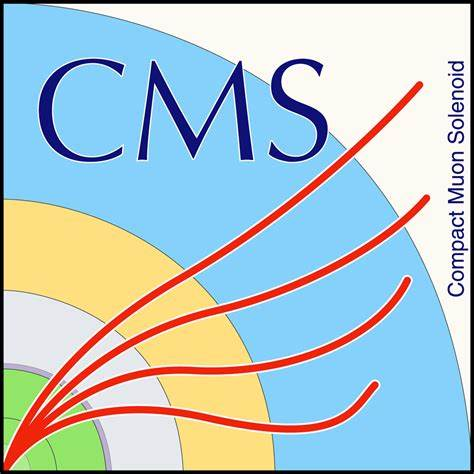
\includegraphics[width=1.5cm]{CMS_logo.jpg}
    % \hspace{2cm}
    
\includegraphics[width=1.5cm]{FNAL_Logo.png}
    % \hspace{2cm}
    \hfill
    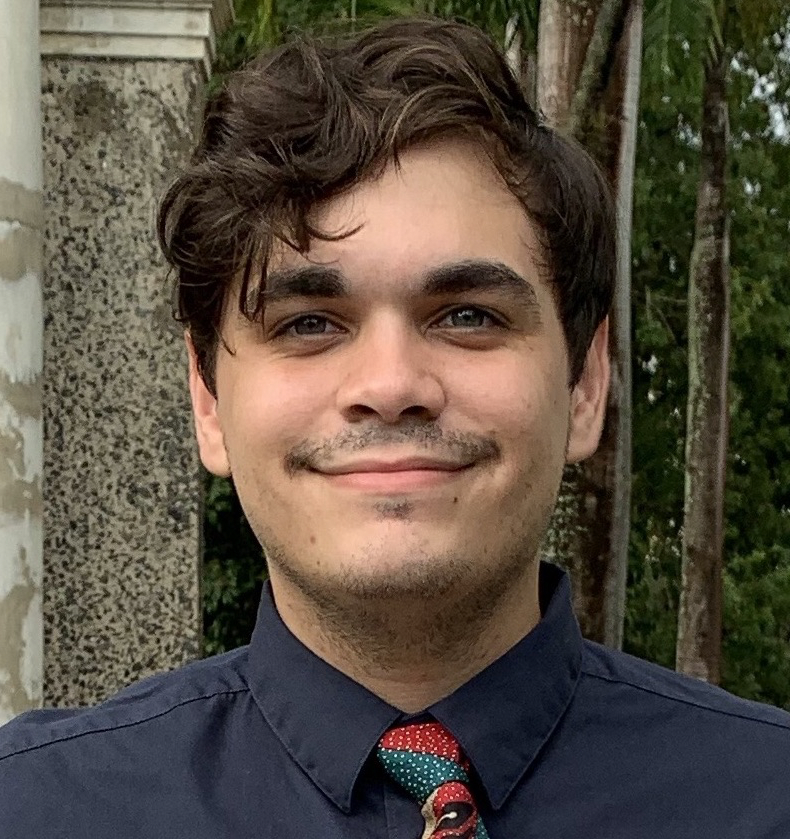
\includegraphics[width=2.7cm]{Guillermo-Grad.png}
}

\begin{document}

\maketitle

\begin{frame}
	\Large
	\tableofcontents
\end{frame}

\section{Introduction}

\begin{frame}{Standard Model of Particle Physics}
	\begin{columns}

		\column{.5\textwidth}
		\begin{itemize}
			\item The most successful theory we have
			      \vspace*{1cm}
			\item Predicted the infamous Higgs Boson discovered in 2012
			      \vspace{1cm}
			\item Not complete, we still have more questions
		\end{itemize}
		\column{.5\textwidth}
		\begin{figure}
			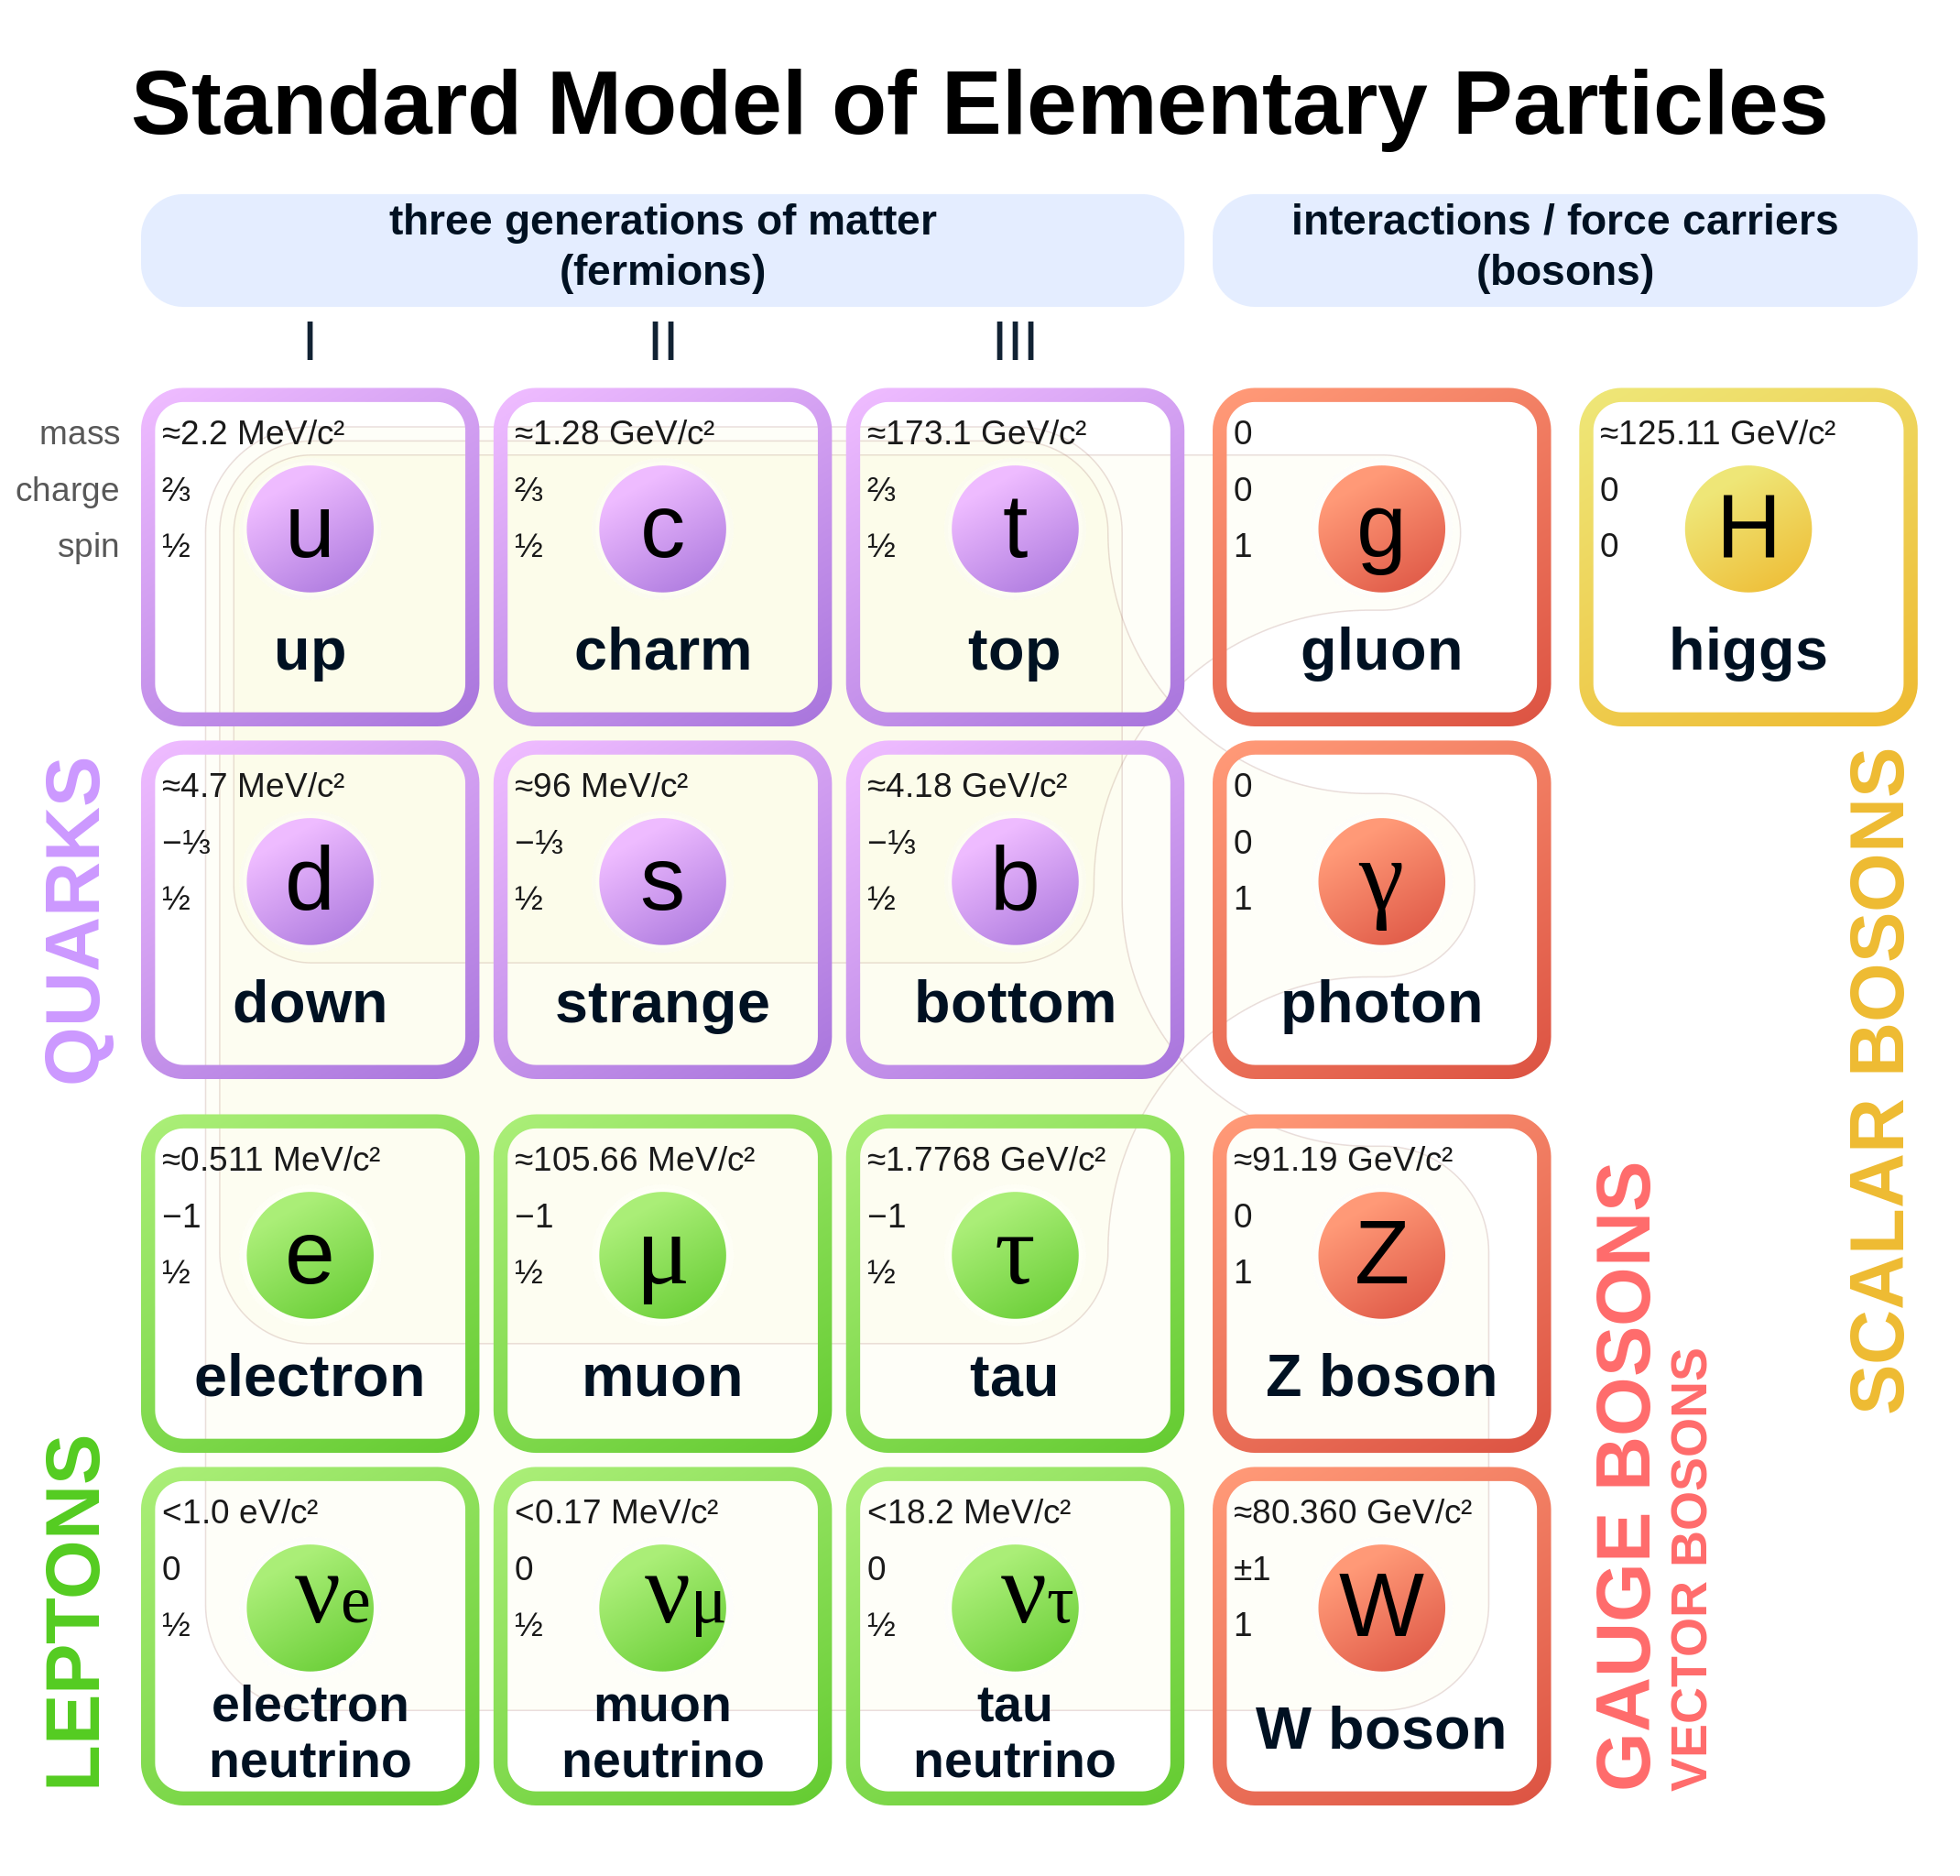
\includegraphics[width=\linewidth]{Standard_Model.png}
		\end{figure}
	\end{columns}
\end{frame}

\begin{frame}{What do we want to accomplish?}
	\begin{itemize}
		\item We want to explain why so much of our Universe is filled with exotic kinds of matter and energy
	\end{itemize}
	\begin{figure}
		\centering
		\begin{subfigure}{0.45\linewidth}
			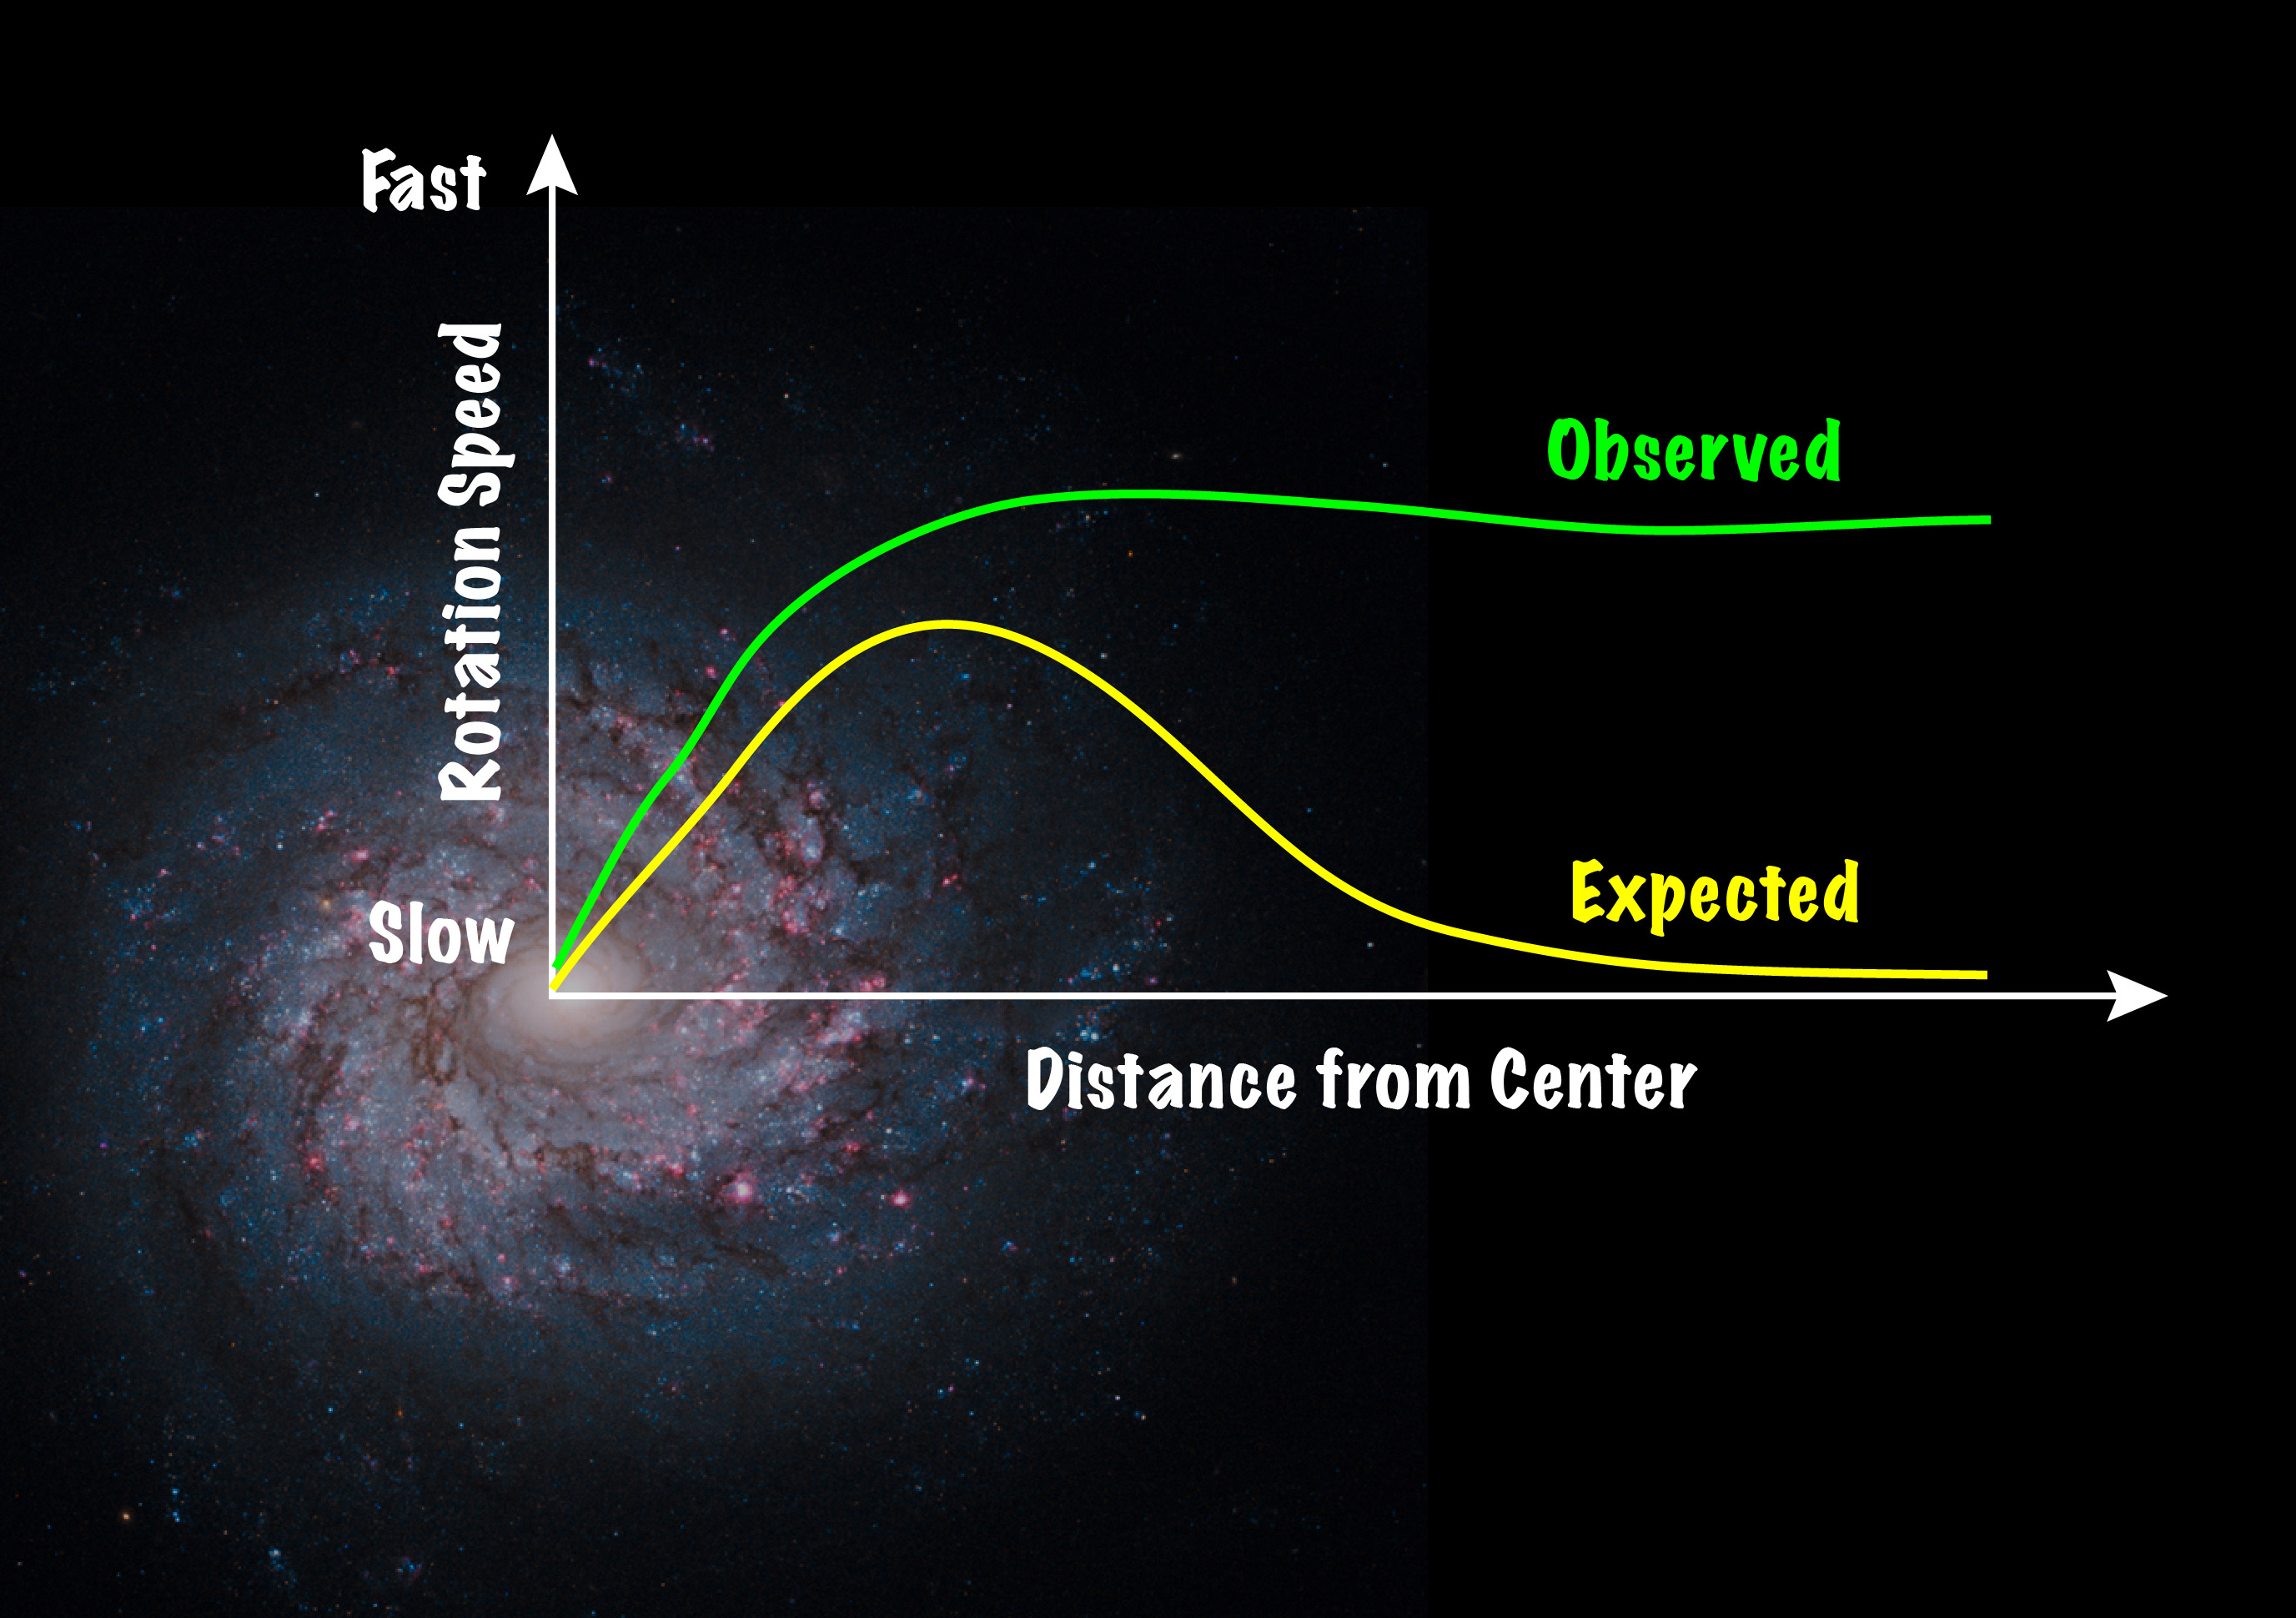
\includegraphics[width=\linewidth]{galaxyrotationcurve.jpg}
			% \caption{Expected vs Observed rotational speed of mass in a galaxy w.r.t. distance from galaxy center.}
		\end{subfigure}
		\begin{subfigure}{0.45\linewidth}
			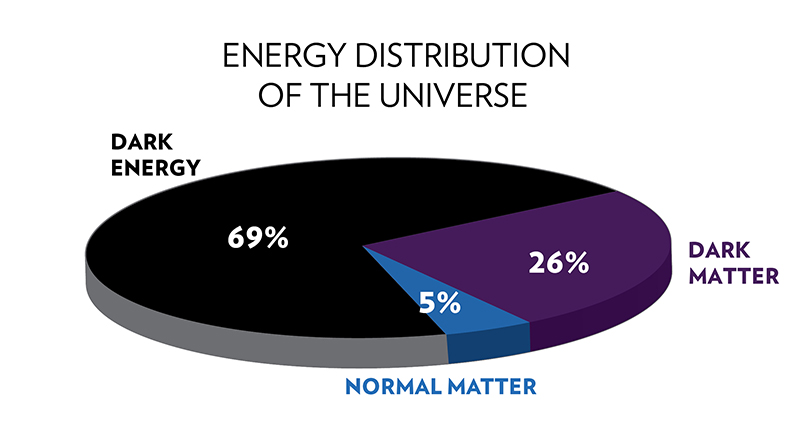
\includegraphics[width=\linewidth]{Energy_dist_pie.jpg}
		\end{subfigure}
	\end{figure}
\end{frame}

\begin{frame}{How do we accomplish it?}
	\begin{columns}
		\column{.45\linewidth}
		\begin{itemize}
			\item In Particle Physics, scientists use the most complex machinery to explore and describe the universe
			\item We accelerate protons to near light-speed to simulate energies of the Big Bang
		\end{itemize}
		\begin{figure}
			\centering
			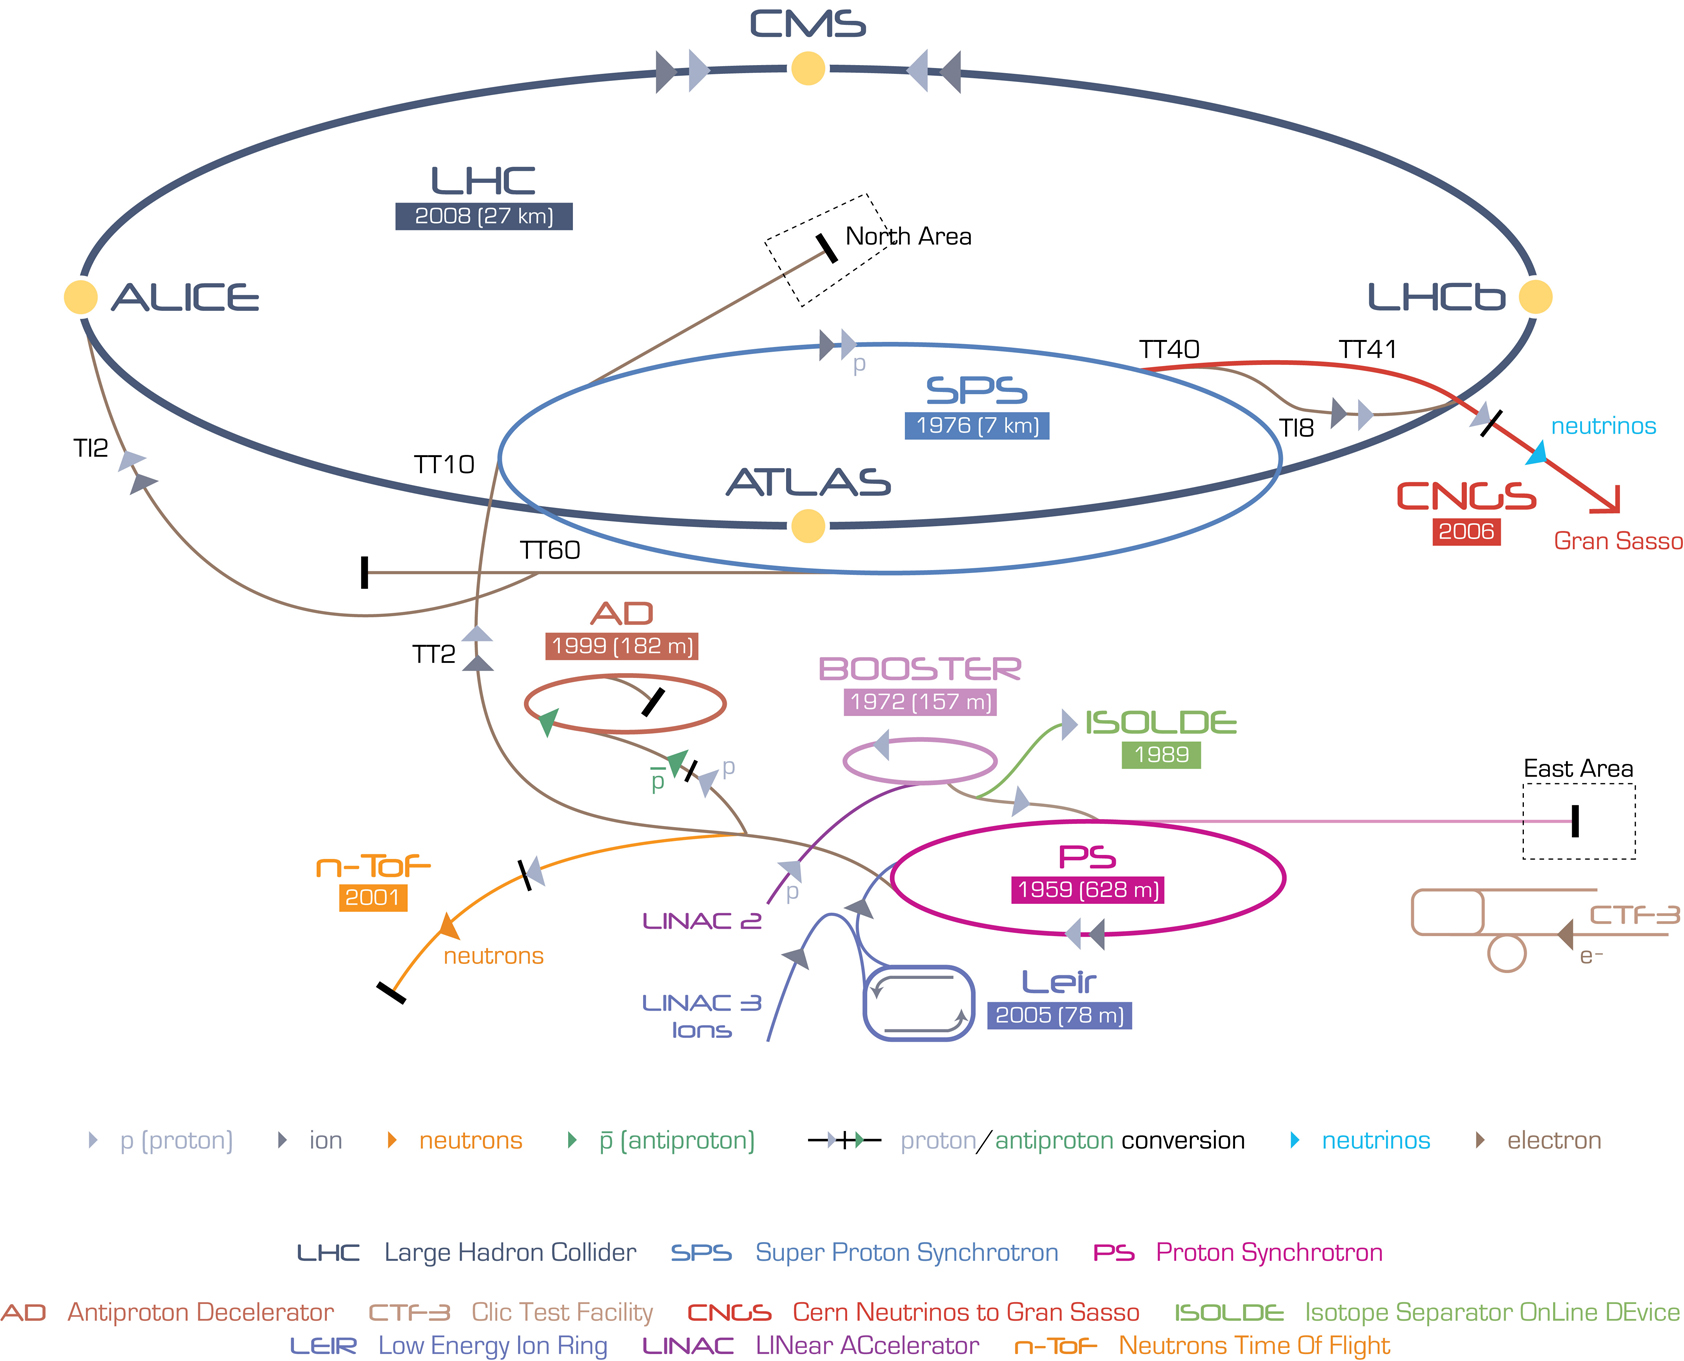
\includegraphics[width=\linewidth]{Cern-Accelerator-Complex.jpg}
		\end{figure}
		\column{.56\linewidth}
		\begin{figure}
			\centering
			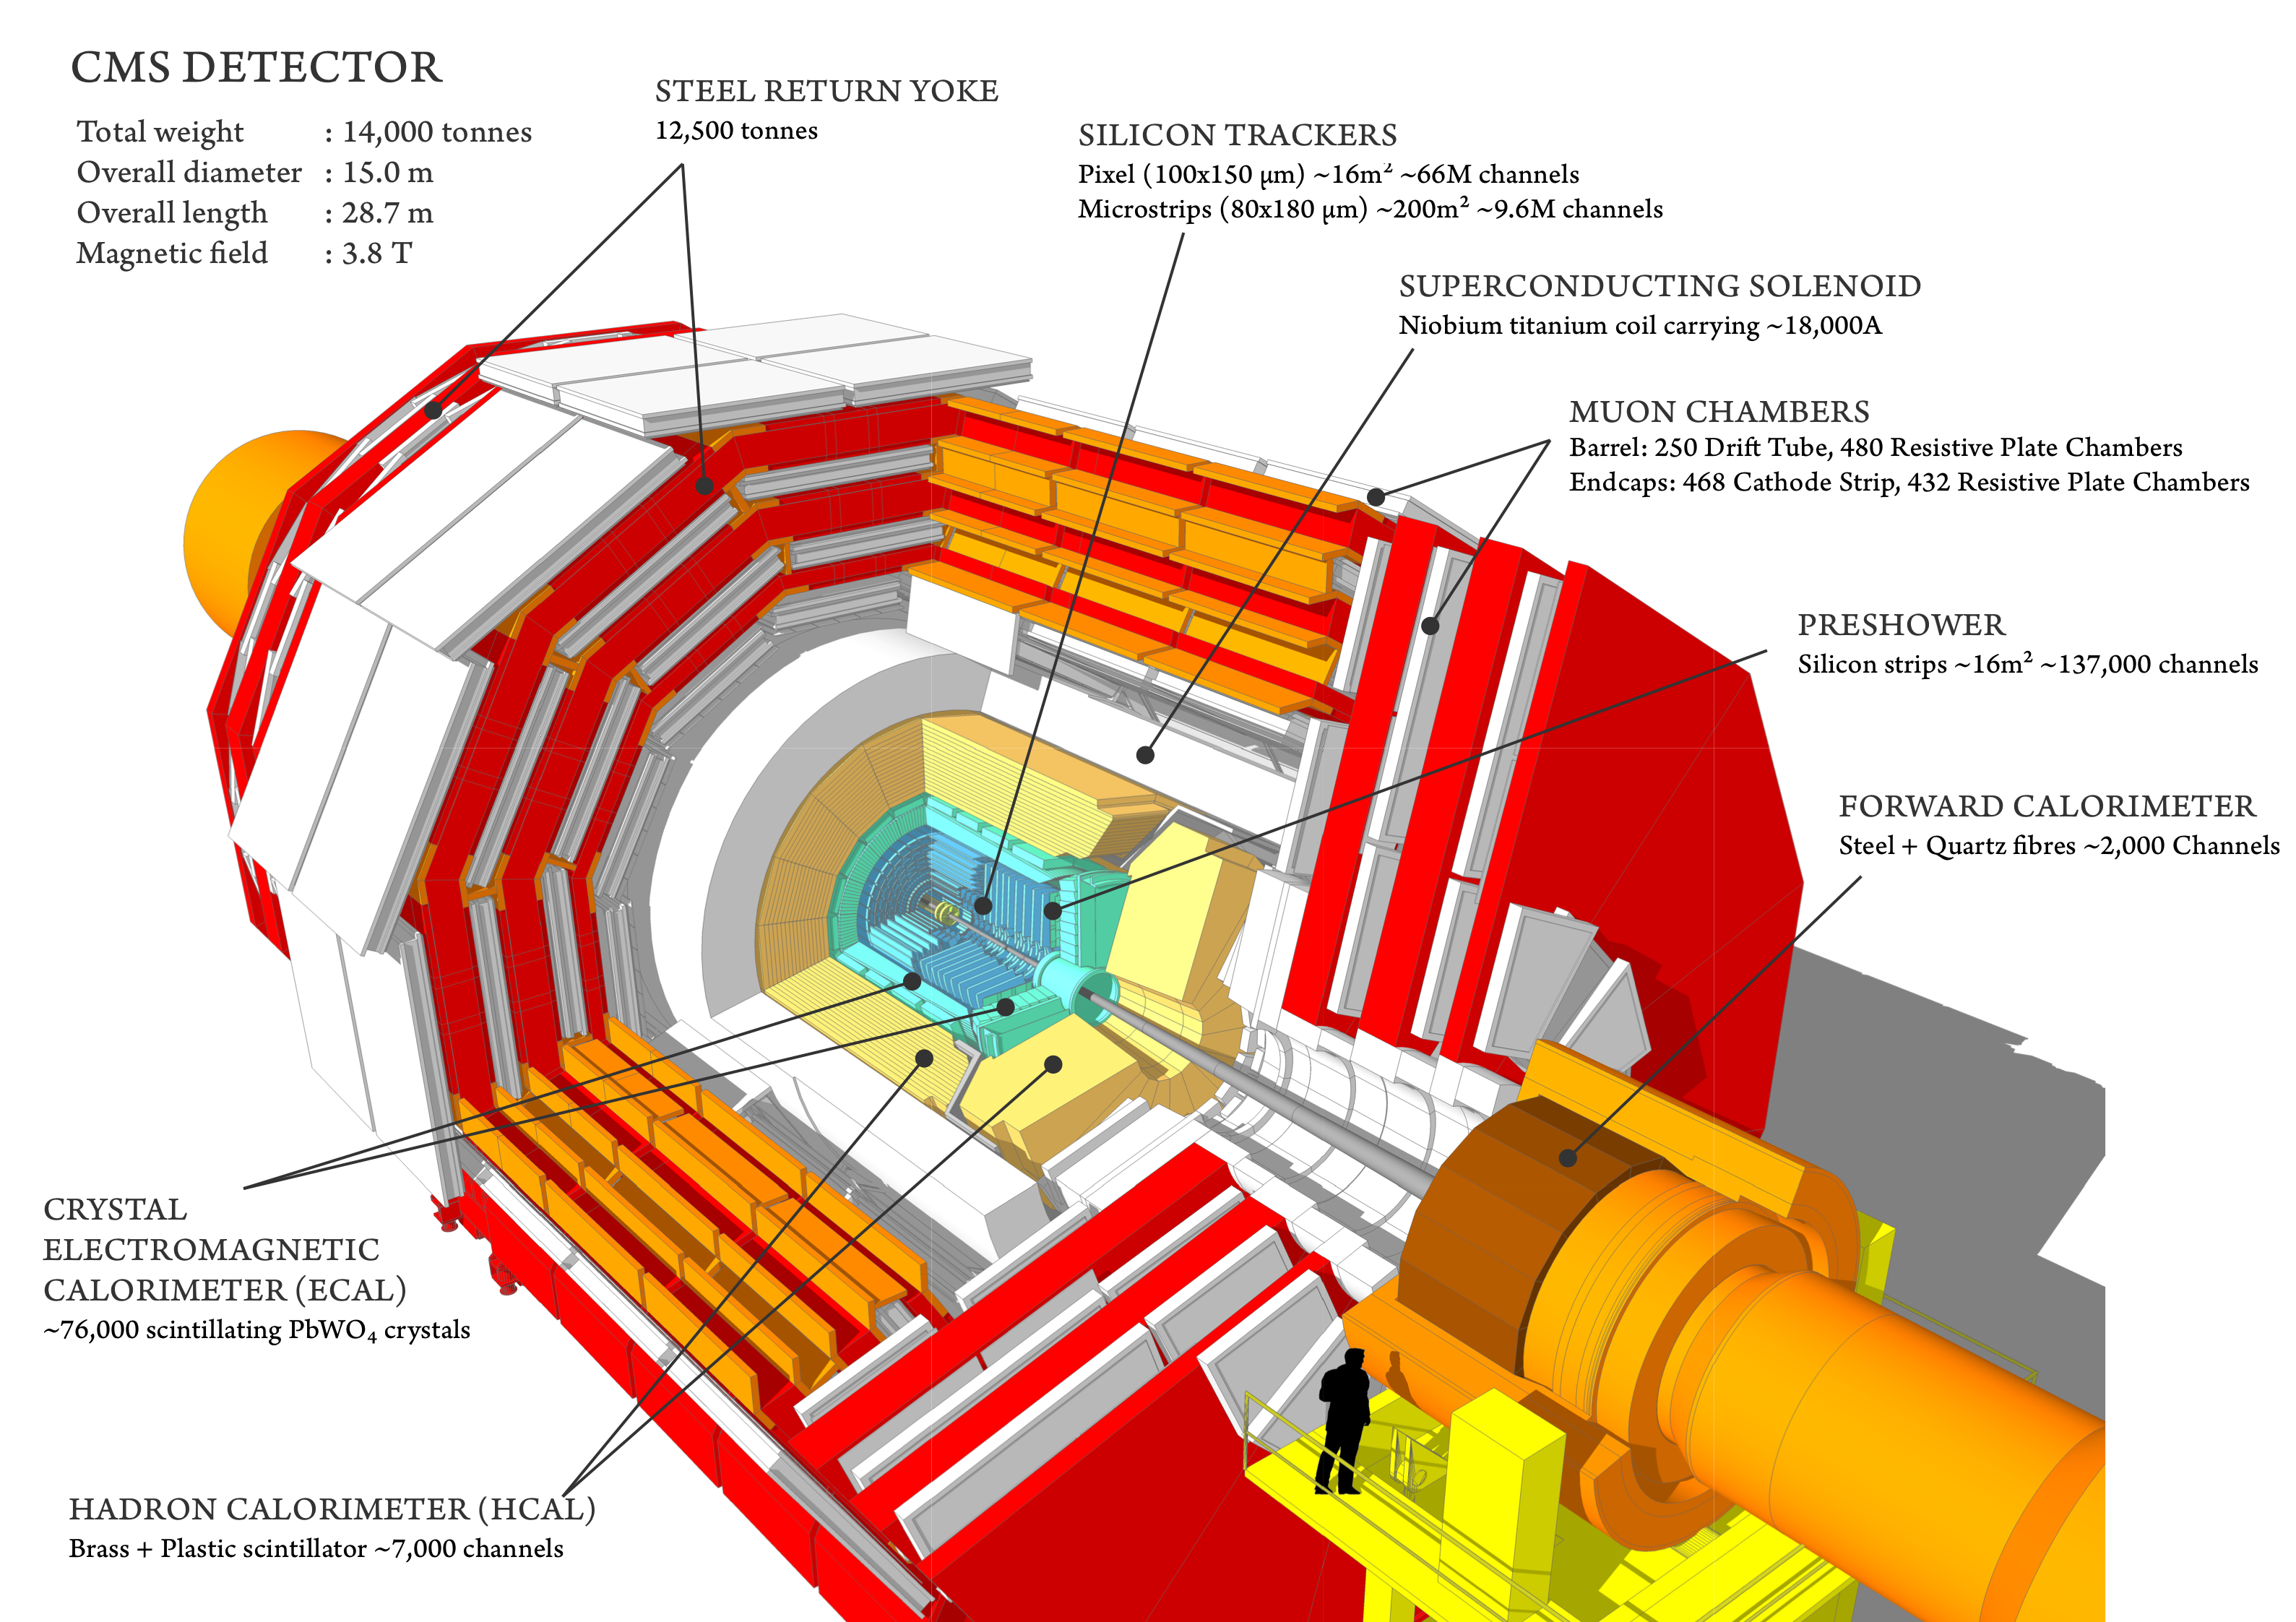
\includegraphics[width=\linewidth]{CMSLayout.png}
		\end{figure}
	\end{columns}
\end{frame}

\begin{frame}{CMS Detector}
	\begin{itemize}
		\item CMS is multipurpose with onion-like structure
		\item Has 3.8 T magnetic field
		\item Precise tracking system
		\item Able to record events at a rate of 40 MHz
	\end{itemize}
	\begin{figure}
		\centering
		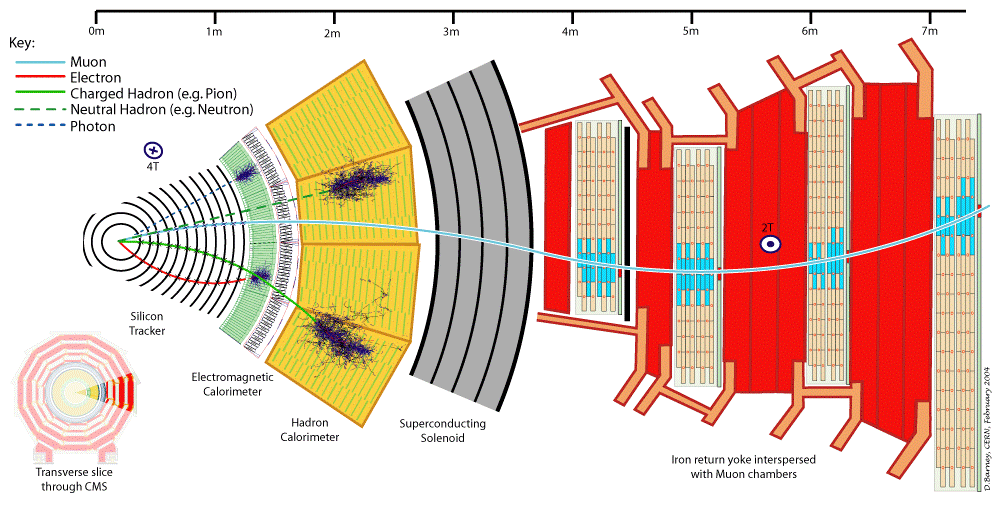
\includegraphics[width=.7\linewidth]{CMSLayers.png}
	\end{figure}
\end{frame}

\begin{frame}
	\frametitle{Trigger System}
	\begin{itemize}
		\item CMS uses a two tier trigger system -- L1 and HLT
	\end{itemize}
	\vfill
	\begin{figure}
		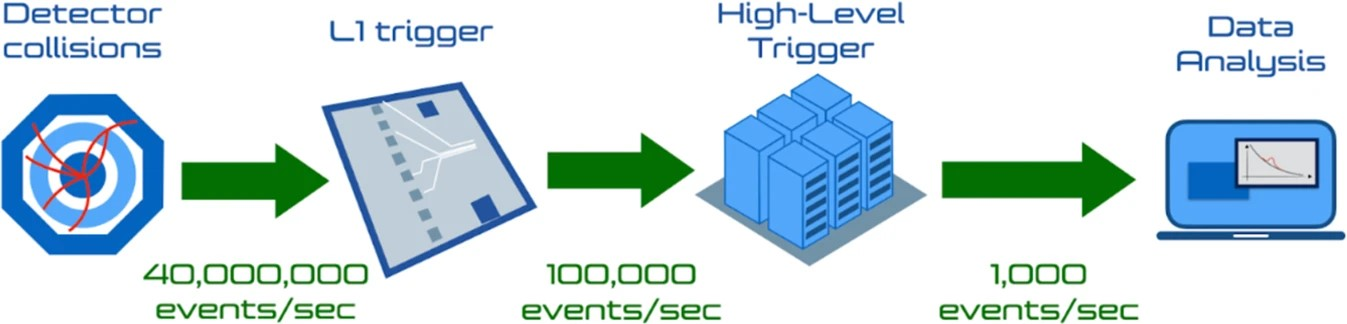
\includegraphics[width=0.8\linewidth]{Trigger_system.jpeg}
	\end{figure}

\end{frame}



\section{Emerging Jets Analysis}

\begin{frame}{EMJ}

\end{frame}

\section{ML4DQM}


\section{Conclusions}



\end{document}
